%===============================================================================
% proj1cdig_relatorio.tex -- Relatório do Prj1CDig (Controle PI Anti-Windup de
% Processo Térmico), grupo 2. Baseado no template OverleafCDig do Prof. Adolfo
% Bauchspiess (adaptado de SBAI/IFAC, ifacconf.cls).
%
% Itens marcados com \pendente{...} (em vermelho) ainda precisam ser preenchidos.
%===============================================================================
\documentclass[a4paper]{ifacconf}

\usepackage{graphicx,amsmath,amssymb,url}
\usepackage[round]{natbib}
\usepackage[brazil,english]{babel}
\usepackage[T1]{fontenc}
\usepackage[utf8]{inputenc}
\usepackage{textcomp}
\usepackage{ae}
\usepackage{xcolor}
\usepackage{booktabs}
\usepackage{listings}
\usepackage{stfloats}   % permite figure* no pé da página
\renewcommand{\dbltopfraction}{0.9}\renewcommand{\textfraction}{0.05}
\renewcommand{\dblfloatpagefraction}{0.85}\setcounter{dbltopnumber}{2}
\setcounter{dblbotnumber}{1}

\newtheorem{teorema}[thm]{{\em Teorema}}{ }

% ----- marcadores de pendência e espaços reservados para fotos -----
\newcommand{\pendente}[1]{\textcolor{red}{[#1]}}
\newcommand{\espacofoto}[2]{%
  \fbox{\parbox[c][#1][c]{0.92\columnwidth}{\centering\small\textcolor{red}{#2}}}}

% ----- listagens de código (anexo) -----
\lstset{basicstyle=\ttfamily\scriptsize, breaklines=true, columns=fullflexible,
  keepspaces=true, numbers=left, numberstyle=\tiny, numbersep=4pt, xleftmargin=12pt, frame=single, showstringspaces=false,
  commentstyle=\color{gray}, extendedchars=true,
  literate=
  {°}{{\textdegree}}1 {µ}{{$\mu$}}1 {·}{{$\cdot$}}1 {É}{{\'E}}1 {Á}{{\'A}}1
  {á}{{\'a}}1 {â}{{\^a}}1 {ã}{{\~a}}1 {à}{{\`a}}1 {ç}{{\c{c}}}1 {é}{{\'e}}1 {ê}{{\^e}}1
  {í}{{\'i}}1 {ó}{{\'o}}1 {õ}{{\~o}}1 {ú}{{\'u}}1 {Ω}{{$\Omega$}}1 {—}{{---}}1 {–}{{--}}1
  {§}{{\S}}1 {±}{{$\pm$}}1 {²}{{$^2$}}1 {×}{{$\times$}}1 {→}{{$\to$}}1 {−}{{-}}1
  {≈}{{$\approx$}}1 {ζ}{{$\zeta$}}1 {ω}{{$\omega$}}1}

\begin{document}
\selectlanguage{brazil}

\begin{frontmatter}

\collab{ENE0167 2026.2 Controle Digital -- Prof. Adolfo Bauchspiess}

\title{Controle PI Anti-Windup Digital de Processo Térmico com ESP32 -- Grupo 2}

\author[First]{Pedro \pendente{Sobrenome}}
\author[Second]{\pendente{Nome do colega}}

\address[First]{\pendente{Matrícula}, \pendente{Curso}, UnB, pviana2000@gmail.com}
\address[Second]{\pendente{Matrícula}, \pendente{Curso}, UnB, \pendente{e-mail}}

\selectlanguage{english}
\renewcommand{\abstractname}{{\bf Abstract:~}}
\begin{abstract}
A digital anti-windup PI controller was identified, designed and implemented on an ESP32 for a
thermal process (LM35 heated by PWM-driven resistors, with a fan as disturbance). The plant was
identified from a 9-hour PRBS experiment and the controller was designed by root locus with
$T_s=T_d/2$. Experiments with and without anti-windup show overshoot of about 0\,\% versus
13--22\,\% in saturated 10\,°C reference steps.

\vskip 1mm
\selectlanguage{brazil}
{\noindent \bf Resumo}: Este relatório descreve a montagem, a identificação, o projeto e a
implementação de um controlador PI digital com anti-windup para um processo térmico formado por
um sensor LM35 aquecido por três resistores acionados por PWM de 16 bits em uma ESP32, com um
cooler como perturbação. O modelo P2DZ foi identificado (\texttt{procest}) a partir de uma coleta
PRBS de 9,07\,h em torno do ponto de operação de 50\,°C, com fit de 86\,\% na validação. O PI foi
projetado no lugar das raízes discreto com $T_s=T_d/2=2{,}629$\,s para $M_p=10\,\%$ e $t_p=25$\,s.
A saturação do atuador foi escolhida experimentalmente ($U_{max}=21000$ contagens) para que a
referência de 60\,°C fosse alcançável mesmo com a perturbação, mas os degraus ainda saturassem.
No ensaio da Figura 5 do roteiro, o anti-windup reduziu o sobrepasso de 13--22\,\% para menos de
1\,\%, com ISE de 2998\,°C$^2\cdot$s (faixa típica: 2000--4000). A perturbação constante foi
rejeitada sem erro em regime; a triangular deixou erro residual de até $\pm$0,8\,°C, limite
esperado de um controlador com um único integrador.
\end{abstract}

\selectlanguage{english}
\begin{keyword}
Digital control; PI controller; anti-windup; system identification; thermal process; ESP32.

\vskip 1mm
\selectlanguage{brazil}
{\noindent\it Palavras-chaves:} controle digital; PI anti-windup; identificação PRBS; lugar das
raízes; processo térmico; ESP32.
\end{keyword}
\selectlanguage{brazil}
\end{frontmatter}

%===============================================================================
\section{Introdução}

O objetivo do Prj1CDig \citep{Bauchspiess:Prj1CDig} é identificar um processo térmico em malha
aberta e controlá-lo com um PI digital anti-windup projetado pelo lugar geométrico das raízes
(LGR), verificando o projeto em simulação e experimentalmente. As especificações do grupo~2 estão
na Tabela~\ref{tb:espec}.

\begin{table}[hb]
\begin{center}
\caption{Especificações do grupo 2 e requisitos do roteiro.}\label{tb:espec}
\begin{tabular}{ll}\toprule
Ponto de operação (P.O.) & 50\,°C \\
Sobrepasso $M_p$ & 10\,\% \\
Tempo de pico $t_p$ & 25\,s \\
Amostragem da identificação $T_i$ & 1\,s \\
Amostragem do controle $T_s$ & $T_d/2$ \\
Resolução da temperatura & $\le 0{,}1$\,°C \\
Perturbações & constantes e triangulares \\
Frequência do cooler $\omega_0$ & 0,065\,rad/s \\ \bottomrule
\end{tabular}
\end{center}
\end{table}

%===============================================================================
\section{Montagem e Instrumentação}\label{sec:montagem}

\subsection{Componentes e ligações}

A bancada segue o item~1 do procedimento do roteiro (Tabela~\ref{tb:componentes} e
Figura~\ref{fig:fotos}). Os três resistores de 150\,$\Omega$ ficam em paralelo, encostados ao
encapsulamento do LM35 do processo para melhorar a transferência de calor. O LM35 do ambiente
fica a cerca de 15\,cm do aquecedor, fora do fluxo de ar do cooler, como pede o roteiro
(``a temperatura ambiente deve ser medida longe da perturbação''). A montagem fica exposta ao
ar da sala, sem caixa, para que o modelo inclua a influência do ambiente.

\begin{table}[hb]
\begin{center}
\caption{Componentes e ligações da bancada.}\label{tb:componentes}
\begin{tabular}{p{2.6cm}p{5.0cm}}\toprule
Item & Especificação / ligação \\ \midrule
Microcontrolador & ESP32-WROOM-32 DevKit, ESP-IDF v6.1 \\
Sensor do processo $T_p$ & LM35, saída no GPIO35 (ADC1\_CH7) \\
Sensor ambiente $T_a$ & LM35, saída no GPIO34 (ADC1\_CH6) \\
Alimentação dos LM35 & 5\,V da USB (4,66\,V medidos) \\
Aquecedor & 3\,$\times$\,150\,$\Omega$, 1/4\,W, em paralelo (50\,$\Omega$), 12\,V \\
PWM do aquecedor & GPIO25, LEDC 16 bits, 1\,kHz \\
Cooler (perturbação) & 12\,V, PWM no GPIO26, 10 bits, 25\,kHz \\
Chaveamento & \pendente{modelo dos transistores} \\
Damper RC nos LM35 & 75\,$\Omega$ (2\,$\times$\,150\,$\Omega$ em paralelo) + 1\,$\mu$F \\
Fonte & 12\,V\,DC \\ \bottomrule
\end{tabular}
\end{center}
\end{table}

\begin{figure}[hbt]
 \begin{center}
  \espacofoto{4.2cm}{Foto da bancada completa (ESP32, protoboard, fonte, cooler, sensores)}\\[1mm]
  \espacofoto{4.2cm}{Foto do detalhe: resistores encostados no LM35 do processo e posição do cooler}
 \caption{Bancada do processo térmico. \pendente{inserir fotos}}
 \label{fig:fotos}
 \end{center}
\end{figure}

\subsection{Medição de temperatura e filtros}

\textbf{Damper RC.} Cada LM35 tem na saída um resistor de 75\,$\Omega$ em série com um capacitor
de 1\,$\mu$F para o terra. É o circuito ``R-C damper'' do datasheet \citep{TI:LM35}, recomendado
quando a saída do sensor alimenta cabos ou cargas capacitivas e há fontes de ruído próximas
(o motor do cooler e o PWM do aquecedor). Sua frequência de canto,
$1/(2\pi\cdot 75\cdot 10^{-6})\approx 2{,}1$\,kHz, está muito acima da dinâmica térmica: ele
estabiliza o sensor, mas não é o filtro do sinal.

\textbf{Filtragem digital.} A filtragem é feita no firmware: cada amostra é a média de 400\,ms
de conversões do ADC1 (cerca de 1600 leituras por sensor). A janela de 400\,ms contém um número
inteiro de ciclos de 50\,Hz (20) e de 60\,Hz (24), que se cancelam na média, e a fase de cada
rajada de leituras é sorteada dentro do período de 1\,ms do PWM do aquecedor, evitando que a
média fique ``presa'' sempre no mesmo ponto da onda.

\textbf{ADC.} Usa-se o ADC1 (o ADC2 conflita com o rádio) com atenuação de 2,5\,dB, cuja faixa
útil (até $\approx$1250\,mV, ou 125\,°C) cobre com folga o limite de segurança de 95\,°C; com
0\,dB a faixa terminaria perto desse limite. A curva de calibração de fábrica gravada em eFuse é
uma reta, $V\,[\mathrm{mV}] = 0{,}31033\,\mathrm{raw} + 77{,}83$, aplicada à média em ponto
flutuante para não perder a resolução ganha na média \citep{Espressif:IDF}. Um LSB vale
0,31\,mV, ou 0,031\,°C.

\textbf{Resultado.} Com o aquecedor desligado, o desvio-padrão de $T_p$ nas últimas 100 amostras
foi de 0,047\,°C (0,036\,°C com o cooler ligado), já incluindo a deriva lenta do ambiente.
Atende ao requisito de resolução de 0,1\,°C sem conversor externo.

\subsection{Atuadores}

\textbf{Aquecedor, PWM de 16 bits.} O roteiro pede PWM de 16 bits (item~2) para ``evitar
propagação de erro''. No LEDC da ESP32, 16 bits exigem $f\le 80\,\mathrm{MHz}/2^{16}=1{,}22$\,kHz,
por isso se usa 1\,kHz, muito acima da banda térmica. Com o ganho identificado
(Seção~\ref{sec:ident}), uma contagem de 16 bits muda $T_p$ em $\approx$0,002\,°C. Com 10 bits
seria $\approx$0,1\,°C por passo, da ordem da resolução exigida, o que levaria o PI a um
ciclo-limite entre dois valores vizinhos. O sinal $u$ é tratado em contagens (0--65535) em todo
o projeto, como na tabela de variáveis do roteiro.

\textbf{Cooler.} PWM de 10 bits a 25\,kHz, a frequência usual de ventoinhas, fora da faixa
audível. Medida a zona morta: o motor parte em $w\approx 530$ (52\,\%). As perturbações usam
$w\in[560;680]$: constante em 680 e triangular $w=620+60\cdot\frac{2}{\pi}\arcsin(\sin\omega_0 t)$,
com período $2\pi/\omega_0=96{,}7$\,s. Em malha aberta a 50\,°C, $w=680$ baixou $T_p$ de 49,7
para 45,3\,°C em 6\,min, tendendo a $\approx$5\,°C de queda.

\subsection{Saturação do atuador}\label{sec:sat}

Cada resistor dissipa $P_R=d\cdot 12^2/150=0{,}96\,d$\,W, sendo $d$ o ciclo de trabalho. O
limite $U_{max}$ (o ``Sat'' do roteiro, usado igualmente no firmware e no MATLAB) foi escolhido
em três etapas (Tabela~\ref{tb:sat}). A conclusão é que ele precisa ficar numa janela:
\begin{equation}\label{eq:janela}
 u_{\text{regime,máx}} < U_{max} < u_{\text{pico}} ,
\end{equation}
onde $u_{\text{regime,máx}}$ é o $u$ que mantém 60\,°C com o cooler em 680 e
$u_{\text{pico}}\approx u_0+K\cdot 10$\,°C é o que o PI pede no instante de um degrau de
10\,°C. Abaixo da janela a referência não é alcançada; acima dela o atuador nunca satura e o
efeito do anti-windup não aparece.

\begin{table}[hb]
\begin{center}
\caption{Escolha experimental de $U_{max}$.}\label{tb:sat}
\begin{tabular}{p{1.1cm}p{1.2cm}p{5.0cm}}\toprule
$U_{max}$ & $d$\,/\,$P_R$ & Resultado \\ \midrule
17000 & 26\,\% / 0,25\,W & potência nominal. No ensaio da Fig.~5, $u$ ficou preso em 17000 nos patamares de 60\,°C com cooler e $T_p$ parou em 55,5--56,2\,°C (ISE = 9372). \\
34000 & 52\,\% / 0,50\,W & simulação (seção~7 do script): $u_{\text{pico}}\approx 30600<U_{max}$, sem saturação; respostas com e sem anti-windup idênticas. \\
\textbf{21000} & \textbf{32\,\% / 0,31\,W} & teste no pior caso (60\,°C, $w=680$, Fig.~\ref{fig:testesat}): satura 26\,s e depois se mantém em $u\approx19560$ (folga de 7\,\%), com $T_p=59{,}9\pm0{,}1$\,°C. \textbf{Adotado.} \\ \bottomrule
\end{tabular}
\end{center}
\end{table}

\begin{figure}[hbt]
 \begin{center}
  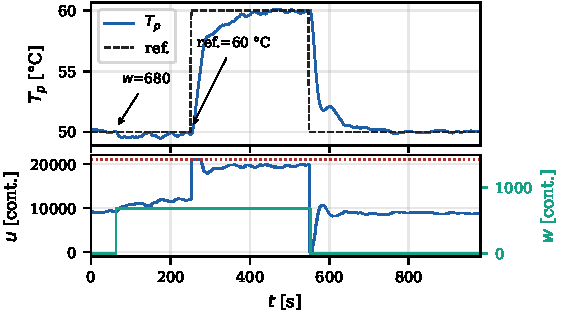
\includegraphics[width=8.4cm]{figs/proj1cdig_teste_saturacao.pdf}
 \caption{Teste do pior caso com $U_{max}=21000$: cooler em 680 a partir de 63\,s e degrau de
 referência para 60\,°C em 252\,s. O atuador satura só no transitório.}
 \label{fig:testesat}
 \end{center}
\end{figure}

O firmware também desliga o aquecedor se $T_p>95$\,°C.

\subsection{Firmware e aquisição}

O firmware (ESP-IDF, Apêndice~\ref{ap:codigo}) tem cinco modos selecionados por comandos na
serial: sensores, malha aberta, PRBS, malha fechada e o perfil de ensaio da Fig.~5 do roteiro,
executado pela própria ESP com o cálculo do ISE. A amostragem é de 1\,s na identificação e
$T_s$ no controle. Um script em Python grava cada amostra em CSV e mostra $T_p$, $T_a$, $u$ e $w$
em tempo real. A coleta de 9\,h foi registrada sem nenhuma amostra perdida ou inválida.

%===============================================================================
\section{Identificação do Processo}\label{sec:ident}

\subsection{Ponto de operação e excursão}

Em malha aberta, $u=11000$ levou $T_p$ a 52,1\,°C, $u=10000$ a 49,6\,°C e $u=10200$ a 49,8\,°C
($T_a\approx27{,}8$\,°C), com 15--20\,min de espera em cada valor. Adotou-se $u_0=10200$
(15,6\,\% de duty). Desses pontos, o ganho local é $\approx$0,0025\,°C/contagem, e a excursão
$\Delta u=5/0{,}0025=2000$ produz os $\pm5$\,°C pedidos no item~2 do roteiro.

\subsection{Coleta PRBS}

O PRBS é gerado na ESP por um registrador de deslocamento de 9 bits com polinômio
$x^9+x^5+1$, que produz a sequência de comprimento máximo de 511 bits. Cada bit dura 60\,s, o
que gera patamares de 60 a 540\,s e excita tanto o polo rápido quanto o lento. O aquecedor
alterna entre $u_0\pm\Delta u$ (8200 e 12200). Antes da sequência, $u$ fica 2000\,s em $u_0$,
trecho descartado na identificação (\texttt{transit} = 2000, como no script do professor). A
coleta durou $2000+511\cdot60=32660$\,s (9,07\,h), com $T_i=1$\,s (Fig.~\ref{fig:prbs}).

\begin{figure}[hbt]
 \begin{center}
  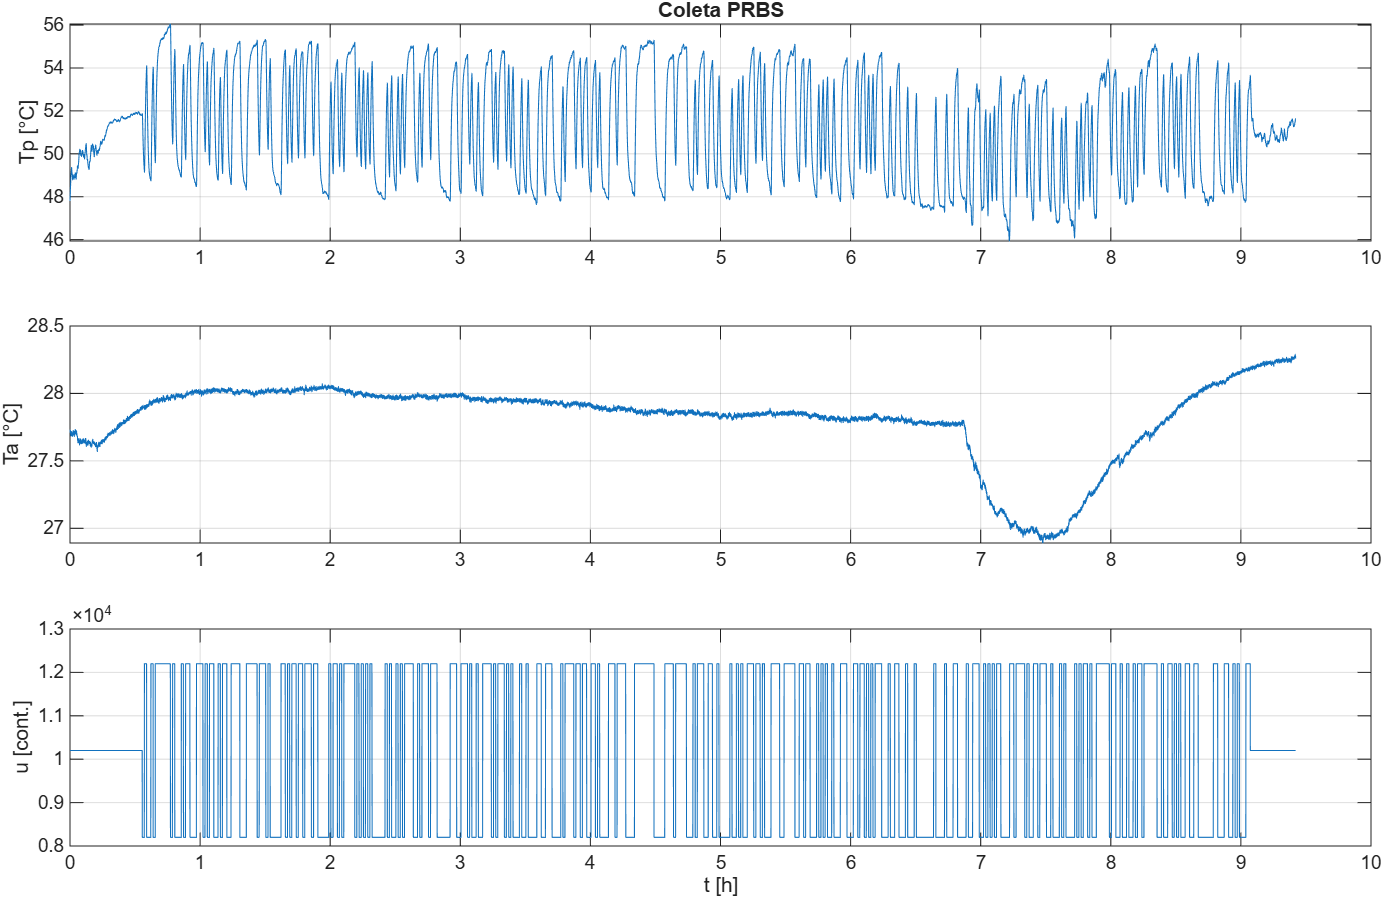
\includegraphics[width=8.4cm]{figs/proj1cdig_coleta_prbs.png}
 \caption{Coleta PRBS: $T_p$, $T_a$ e $u$ (9,07\,h, $u_0=10200$, $\Delta u=2000$).}
 \label{fig:prbs}
 \end{center}
\end{figure}

$T_p$ variou entre 45,9 e 56,1\,°C, com média de 51,3\,°C. A média ficou 1,3\,°C acima do P.O.
porque a convecção natural da madrugada diferiu da noite em que $u_0$ foi medido: com $u$ médio
constante, a média horária de $T_p$ variou entre 49,8 e 52,5\,°C. $T_a$ ficou entre 26,9 e
28,3\,°C, com uma queda de $\approx$0,9\,°C ao amanhecer.

\subsection{Estimação do modelo P2DZ}

O modelo do roteiro é
\begin{equation}\label{eq:p2dz}
G(s)=\frac{T_p(s)}{U(s)}=K_p\frac{1+T_z s}{(1+T_{p1}s)(1+T_{p2}s)}e^{-T_d s}.
\end{equation}
Ele foi estimado com o \texttt{procest} \citep{MathWorks:procest,Ljung:1999}, com três decisões:

\textbf{Saída $T_p-T_a$.} O roteiro modela o efeito do ambiente por
$G_a(s)=T_p(s)/T_a(s)$ com ganho DC unitário. Subtrair $T_a$ remove da identificação as
variações lentas do ambiente, como a queda ao amanhecer, que $u$ não explica.

\textbf{Chute inicial e limites.} Sem valores iniciais, o \texttt{procest} converge para um
mínimo local sem significado físico ($T_z=0$, $T_{p1}\approx38$\,s, $T_{p2}\approx2{,}5$\,s,
$T_d\approx2{,}2$\,s) e fit menor. Iniciou-se em $K_p=0{,}002$ (ganho da etapa anterior),
$T_{p1}=300$\,s, $T_{p2}=40$\,s, $T_z=200$\,s e $T_d=4$\,s (faixas do roteiro), com limites largos
(por exemplo, $50\le T_{p1}\le2000$\,s). Partidas diferentes levaram ao mesmo mínimo.

\textbf{Validação cruzada.} Foram testadas 19 partições identificação/validação e escolhido o
modelo de maior fit em \texttt{compare}.

\begin{table}[hb]
\begin{center}
\caption{Modelo identificado ($y=T_p-T_a$, $u$ em contagens).}\label{tb:modelo}
\begin{tabular}{lll}\toprule
Parâmetro & Valor & Roteiro \\ \midrule
$K_p$ & 0,00320\,°C/cont. & -- \\
$T_z$ & 821,9\,s & $T_{p2}$--$T_{p1}$ \\
$T_{p1}$ & 1553,9\,s & 200--400\,s \\
$T_{p2}$ & 34,46\,s & 20--50\,s \\
$T_d$ & 5,257\,s & 3--8\,s \\
Fit (75\,\% validação) & 86,4\,\% & -- \\ \bottomrule
\end{tabular}
\end{center}
\end{table}

\begin{figure}[hbt]
 \begin{center}
  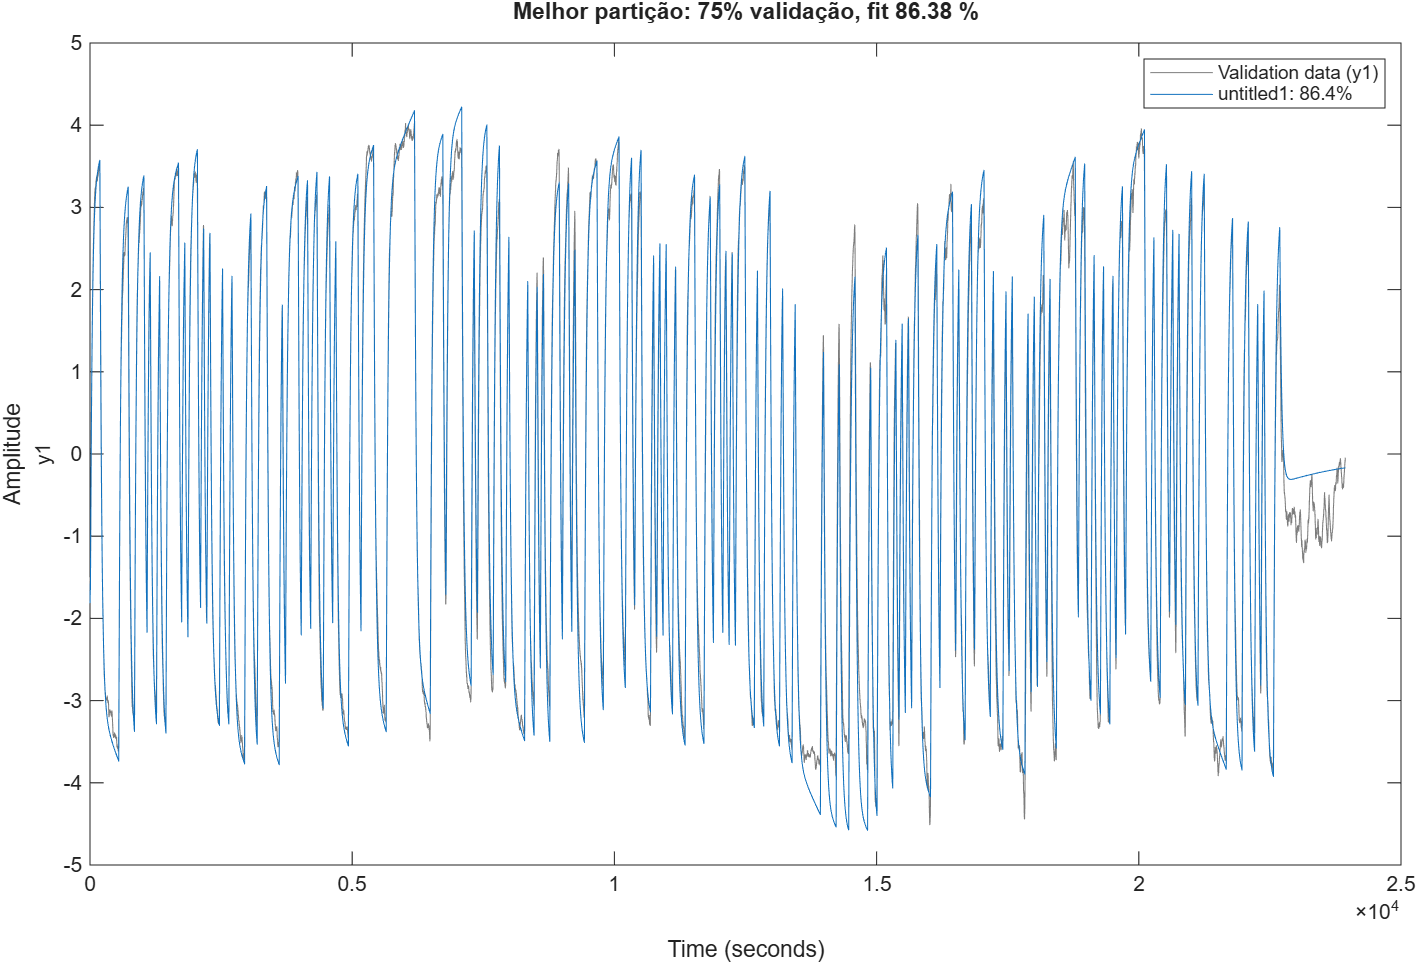
\includegraphics[width=8.4cm]{figs/proj1cdig_validacao.png}
 \caption{Validação: identificação com 25\,\% dos dados, validação nos 75\,\% restantes
 ($y$ sem média). Fit de 86,4\,\%.}
 \label{fig:validacao}
 \end{center}
\end{figure}

O melhor modelo (Tabela~\ref{tb:modelo}, Fig.~\ref{fig:validacao}) foi identificado com só
25\,\% dos dados (2,1\,h) e validado nos 75\,\% restantes. O fit de todas as partições ficou entre
70 e 86\,\%. O modelo reproduz toda a dinâmica rápida; o que fica sem explicação são derivas lentas
da convecção do ar, que nenhuma entrada medida contém.

$T_{p1}$ ficou acima da faixa do roteiro, e o par lento $(T_z,T_{p1})$ é pouco determinado: outras
partições e pontos de partida dão $T_{p1}$ entre $\approx$1500 e 3400\,s com $T_z/T_{p1}\approx0{,}5$
e praticamente o mesmo fit. Sem isolamento, esse modo lento absorve o aquecimento do entorno. Já a
parte rápida, que define o controle, é consistente em todas as variantes:
$K_pT_z/T_{p1}\approx0{,}0017$\,°C/cont., $T_{p2}\approx34$--35\,s e $T_d\approx5{,}2$--5,3\,s. Em
escala de 10 bits ($\times64$), o ganho rápido equivale a 0,11\,°C/contagem, coerente com a faixa
$K_p=0{,}05$--0,1 do roteiro. O PI final, aplicado a três variantes do modelo, dá $M_p$ entre 8,6
e 10\,\% e $t_p=23{,}7$\,s em todas.

%===============================================================================
\section{Projeto do Controlador}

\subsection{Polo dominante}

De $M_p=10\,\%$ e $t_p=25$\,s:
$\zeta=-\ln M_p/\sqrt{\pi^2+\ln^2M_p}=0{,}5912$,
$\omega_n=\pi/(t_p\sqrt{1-\zeta^2})=0{,}1558$\,rad/s, e
$s_d=-0{,}0921\pm j0{,}1257$.

\subsection{PI contínuo (itens 4 e 5 do roteiro)}

Para $C(s)=K_P(s+a)/s$, a condição de ângulo em $s_d$ posiciona o zero em $a=0{,}0679$\,s$^{-1}$
e a de módulo dá $K_P=2150$\,cont./°C ($K_I=K_Pa=145{,}9$\,cont./(°C$\cdot$s)). A simulação linear
desse ponto de partida dá $M_p=38\,\%$ e $t_p=22{,}7$\,s: o zero do PI e os polos adicionais
aumentam o sobrepasso, e o ajuste final é feito no sisotool. \pendente{inserir figura do sisotool
contínuo, valores finais de $K_P$ e $K_I$ e a verificação no Simulink (\texttt{Prj1CDig.slx}) com
saturação e anti-windup}

\subsection{PI discreto (itens 6 e 7)}

\textbf{Período de amostragem.} $T_s=T_d/2=2{,}629$\,s (item~6a). O atraso foi representado como
exatamente duas amostras: com $T_d/T_s$ fracionário (1,997), a discretização ZOH introduz um zero
espúrio muito afastado (em torno de $z\approx-300$), que não altera a resposta mas distorce o LGR.

\textbf{Projeto.} Com $G(z)$ obtida por ZOH, o polo desejado é
$z_d=e^{s_dT_s}=0{,}7425\pm j0{,}2547$. Para
\begin{equation}\label{eq:pid}
C(z)=K\frac{z-z_0}{z-1},
\end{equation}
a condição de ângulo dá $z_0=0{,}8849$ e $K=1935$, com $M_p=27{,}2\,\%$ e $t_p=26{,}3$\,s.
Refinou-se então $(K,z_0)$ por busca em grade em torno desse ponto, minimizando os desvios de
$M_p$ e $t_p$ na resposta ao degrau:
\begin{equation}
K=2039{,}96\ \text{cont./°C},\qquad z_0=0{,}94216,
\end{equation}
com $M_p=10{,}1\,\%$ e $t_p=23{,}7$\,s na simulação linear.
Os polos de malha fechada (Fig.~\ref{fig:lgr}) são $0{,}7033\pm j0{,}3185$ ($\zeta=0{,}52$,
$\omega_n=0{,}189$\,rad/s), $0{,}946$ (quase cancelado pelo zero do PI em 0,942), $0{,}9968$ (quase
cancelado pelo zero da planta) e $-0{,}42$. Os pares polo-zero próximos alteram a resposta: os
polos dominantes ficam um pouco abaixo de $\zeta=0{,}59$ justamente para que a resposta completa
tenha $M_p=10\,\%$. \pendente{inserir figura do sisotool discreto}

\begin{figure}[hbt]
 \begin{center}
  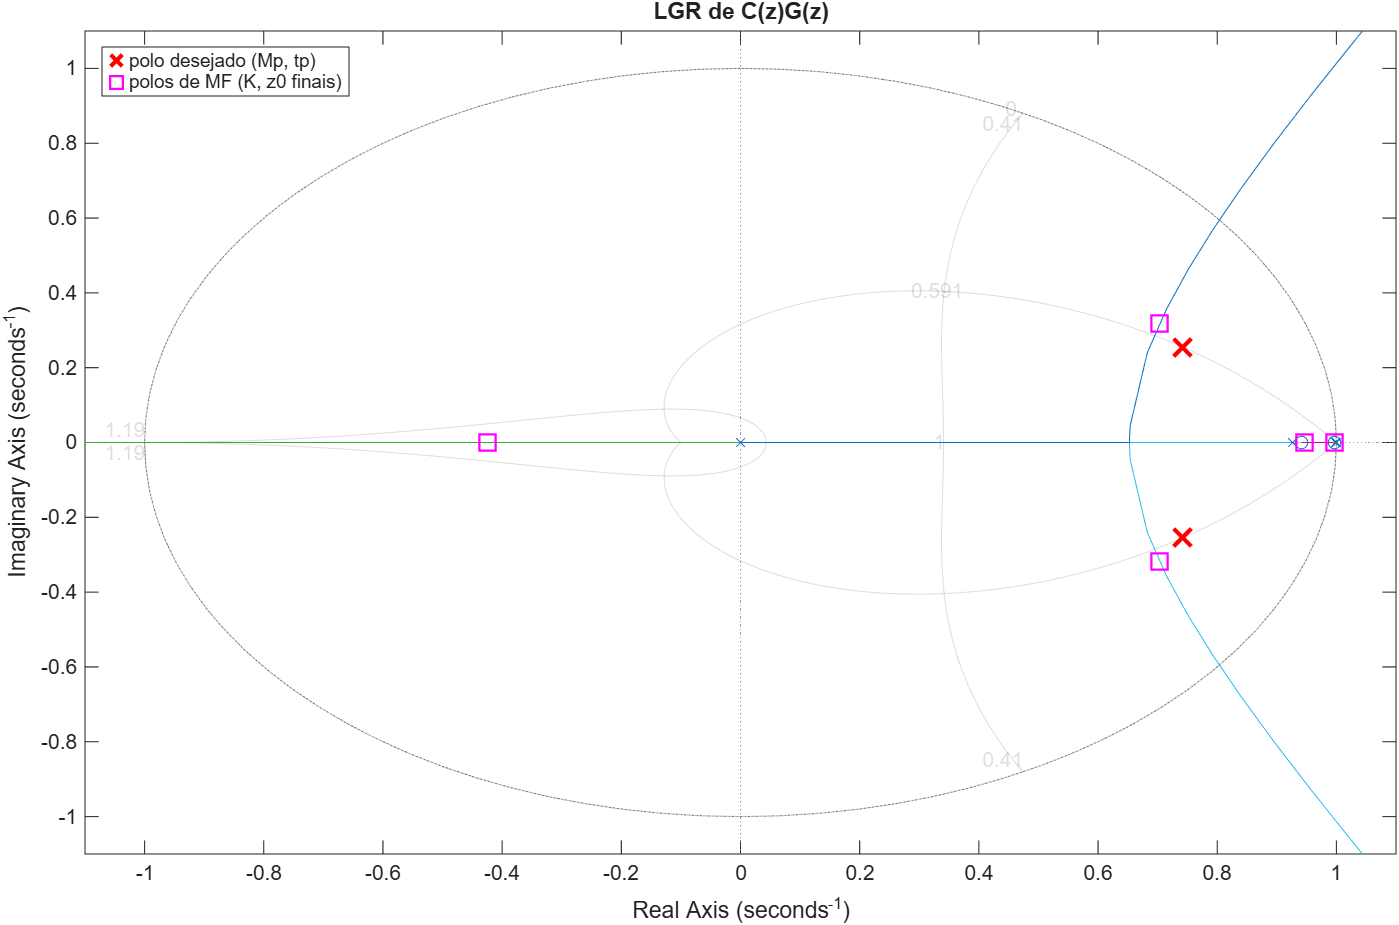
\includegraphics[width=8.4cm]{figs/proj1cdig_lgr_discreto.png}
 \caption{LGR de $C(z)G(z)$ com a grade de $\zeta$ e $\omega_n$: polo desejado ($\times$) e polos
 de malha fechada com o PI final ($\square$).}
 \label{fig:lgr}
 \end{center}
\end{figure}

\textbf{Lei de controle e anti-windup.} O PI é implementado como
\begin{align}
u(k)&=K\,e(k)+I(k),\qquad u_a(k)=\mathrm{sat}_{[0,\,U_{max}]}\big(u(k)\big),\\
I(k+1)&=I(k)+\delta(k)\,K(1-z_0)\,e(k),
\end{align}
que é \eqref{eq:pid} na forma $K+K(1-z_0)/(z-1)$, com $\delta(k)=0$ se o anti-windup está ligado
e ($u>U_{max}$ com $e>0$) ou ($u<0$ com $e<0$), e $\delta(k)=1$ caso contrário. O anti-windup por integração condicional
\citep{AstromHagglund:2006} congela o integrador quando o atuador está saturado e o erro empurra
para mais saturação. Ao entrar em malha fechada, $I$ é iniciado com o $u$ atual (partida sem
solavanco).

\subsection{Simulação com saturação}

A seção~7 do script simula $G(z)$ em torno do ponto de operação medido ($u_0=10200$), com a mesma
lei do firmware (Tabela~\ref{tb:sim}, Fig.~\ref{fig:sim}). No degrau de 10\,°C, o da Fig.~5 do
roteiro, o integrador sem anti-windup acumula durante a saturação e o sobrepasso sobe de 0,5 para
13,5\,\%. No de 5\,°C a saturação dura só 3\,s e a diferença é pequena. \pendente{inserir a
verificação no Simulink (item~7) com o PI discreto}

\begin{table}[hb]
\begin{center}
\caption{Simulação com saturação em $U_{max}=21000$.}\label{tb:sim}
\begin{tabular}{lcccc}\toprule
 & \multicolumn{2}{c}{Com AW} & \multicolumn{2}{c}{Sem AW} \\
Degrau & $M_p$ & satur. & $M_p$ & satur. \\ \midrule
5\,°C & 4,8\,\% & 3\,s & 9,7\,\% & 3\,s \\
10\,°C & 0,5\,\% & 16\,s & 13,5\,\% & 29\,s \\ \bottomrule
\end{tabular}
\end{center}
\end{table}

\begin{figure}[hbt]
 \begin{center}
  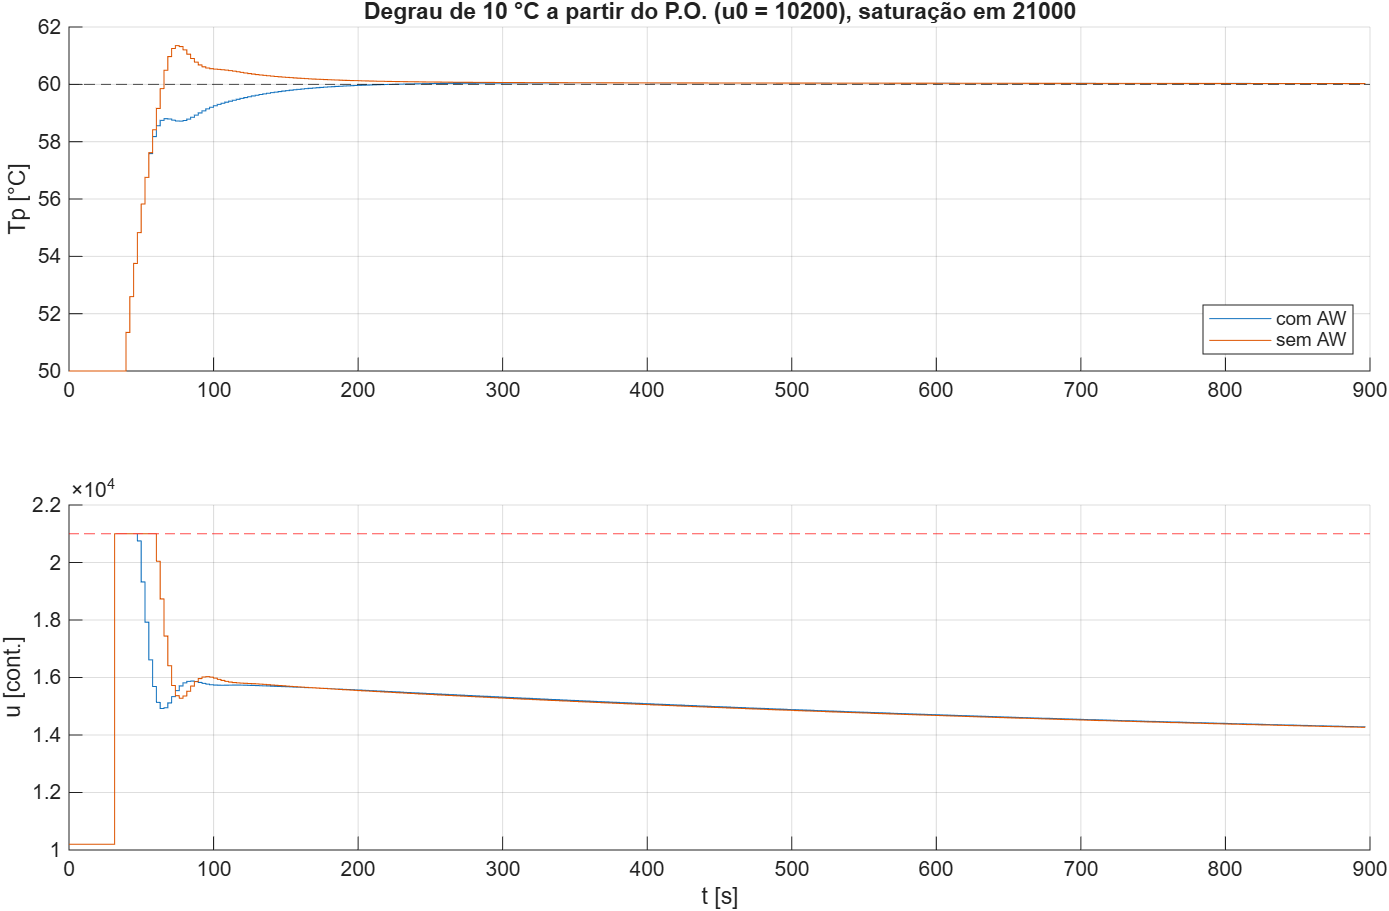
\includegraphics[width=8.4cm]{figs/proj1cdig_sim_aw_10C.png}
 \caption{Simulação do degrau de 10\,°C (50$\to$60\,°C em $t=30$\,s) com saturação em 21000,
 com e sem anti-windup (seção~7 do script).}
 \label{fig:sim}
 \end{center}
\end{figure}

%===============================================================================
\section{Resultados Experimentais}

\subsection{Ensaio do roteiro (Figura 5)}

O perfil do item~8 foi executado pela ESP duas vezes, com e sem anti-windup
(Fig.~\ref{fig:ensaio}): a referência alterna entre 50 e 60\,°C a cada 400\,s; o cooler fica
desligado até 1000\,s, constante em 680 até 1800\,s, triangular até 2600\,s e constante até
3600\,s. O ISE é calculado entre 2100 e 3000\,s.

\begin{figure*}[t]
 \begin{center}
  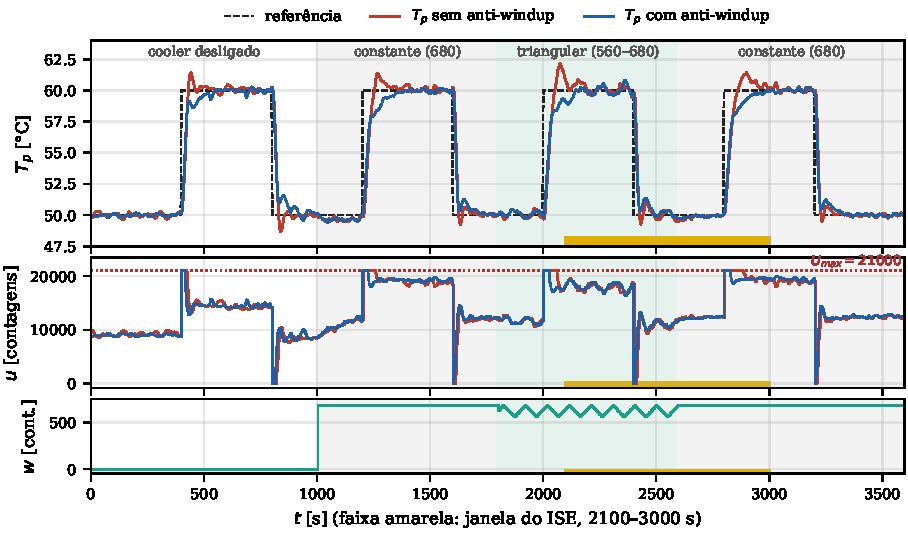
\includegraphics[width=17cm]{figs/proj1cdig_ensaio_aw.pdf}
 \caption{Ensaio do roteiro com e sem anti-windup ($U_{max}=21000$, $K=2040$, $z_0=0{,}942$,
 $T_s=2{,}629$\,s). Fundo cinza: cooler constante; verde: triangular.}
 \label{fig:ensaio}
 \end{center}
\end{figure*}

\begin{figure*}[t]
 \begin{center}
  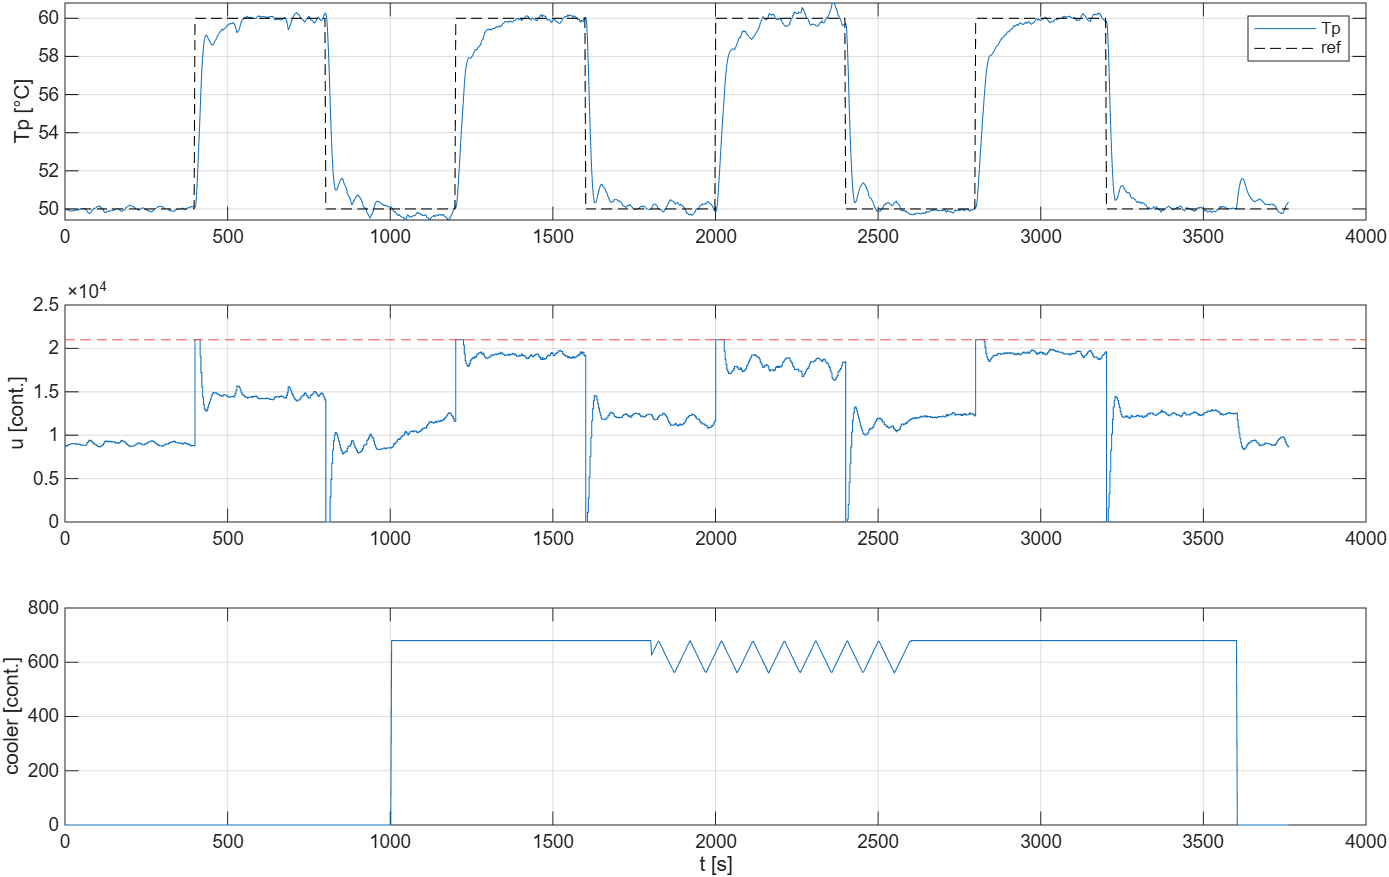
\includegraphics[width=7.4cm]{figs/proj1cdig_malha_fechada_aw1.png}\hspace{6mm}
  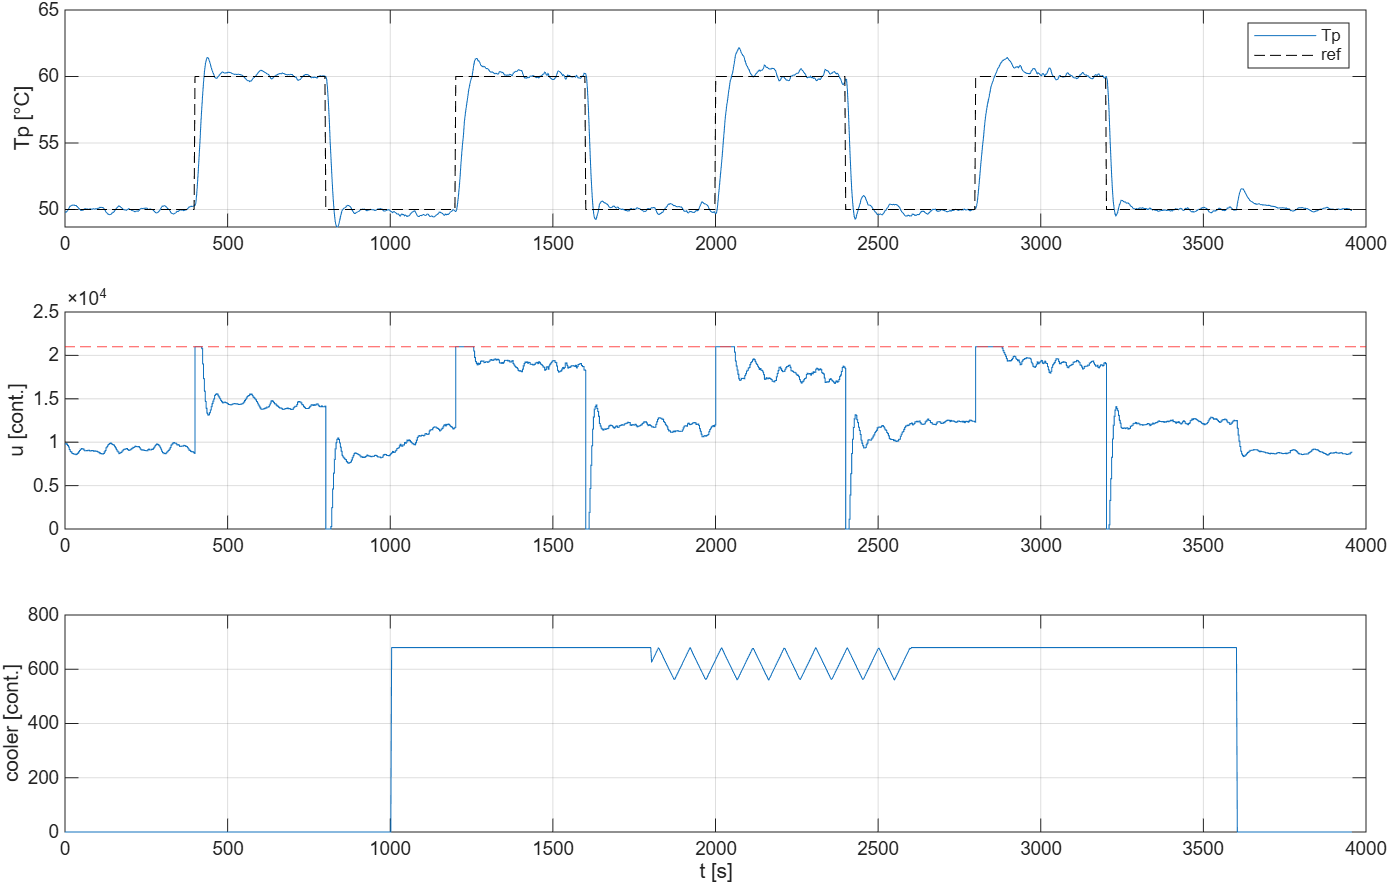
\includegraphics[width=7.4cm]{figs/proj1cdig_malha_fechada_aw0.png}
 \caption{Ensaios analisados pela seção~9 do script: com anti-windup (esquerda) e sem
 anti-windup (direita). De cima para baixo: $T_p$ e referência, $u$ (saturação em 21000,
 tracejado) e cooler.}
 \label{fig:mf}
 \end{center}
\end{figure*}

\begin{table}[hb]
\begin{center}
\caption{Degraus de subida (50$\to$60\,°C): sobrepasso nos primeiros 150\,s, tempo saturado e
tempo até 90\,\% do degrau.}\label{tb:degraus}
\begin{tabular}{llcccccc}\toprule
 & & \multicolumn{3}{c}{Com AW} & \multicolumn{3}{c}{Sem AW} \\
\# & Cooler & $M_p$ & sat. & $t_{90}$ & $M_p$ & sat. & $t_{90}$ \\ \midrule
1 & off & 0,0\,\% & 13\,s & 31\,s & 14,3\,\% & 21\,s & 29\,s \\
3 & 680 & 0,0\,\% & 24\,s & 88\,s & 13,5\,\% & 55\,s & 46\,s \\
5 & tri. & 0,9\,\% & 26\,s & 74\,s & 21,6\,\% & 58\,s & 45\,s \\
7 & 680 & 0,0\,\% & 24\,s & 84\,s & 14,3\,\% & 81\,s & 50\,s \\ \bottomrule
\end{tabular}
\end{center}
\end{table}

\begin{figure}[tb]
 \begin{center}
  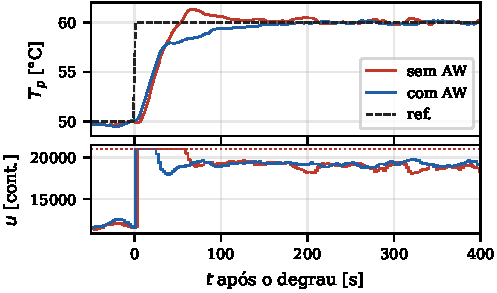
\includegraphics[width=8.4cm]{figs/proj1cdig_degrau3_zoom.pdf}
 \caption{Detalhe do degrau 3 (cooler em 680): sem anti-windup, 55\,s saturado e
 $T_p>61$\,°C.}
 \label{fig:zoom}
 \end{center}
\end{figure}

\textbf{Anti-windup.} Em todos os degraus de subida o atuador saturou em 21000
(Tabela~\ref{tb:degraus}, Fig.~\ref{fig:zoom}). Sem anti-windup, o integrador acumulou erro
durante a saturação: o aquecedor ficou saturado de 1,6 a 3,4 vezes mais tempo e o sobrepasso foi de
13,5 a 21,6\,\%, contra no máximo 0,9\,\% com anti-windup. Nas descidas, que saturam em
$u=0$, o afundamento abaixo de 50\,°C foi de 5 a 13\,\% sem anti-windup e de no máximo 4,8\,\%
com ele. Com anti-windup a chegada final é mais lenta (90\,\% em 74--88\,s com o cooler, contra
45--50\,s sem), porque o integrador congelado precisa voltar a acumular depois que o atuador sai da
saturação.

\textbf{Simulação $\times$ experimento.} No degrau 1 (sem cooler, como na simulação), o sobrepasso
sem anti-windup foi de 14,3\,\% (simulado: 13,5\,\%) e o tempo saturado, de 13\,s com e 21\,s sem
anti-windup (simulado: 16 e 29\,s).

\textbf{ISE.} 2997,7\,°C$^2\cdot$s com anti-windup e 2937,6 sem, ambos na faixa típica do roteiro
(2000--4000). O ISE quase não distingue as duas versões: na janela de 2100 a 3000\,s, a subida
mais rápida sem anti-windup compensa o sobrepasso. $M_p$ e o tempo saturado mostram melhor o
benefício.

\textbf{Verificação no MATLAB.} A seção~9 do script (Tabela~\ref{tb:secao9},
Fig.~\ref{fig:mf}) confirma os valores do firmware. Sem anti-windup, o pico vem 39\,s após o
1º degrau (sobrepasso de fato, 14,3\,\%) e o aquecedor satura 2,3 vezes mais tempo. Com
anti-windup, a seção~9 busca o pico em todo o patamar de 400\,s e encontra a oscilação de
convecção a +313\,s; nos primeiros 150\,s, $T_p$ não passa de 60\,°C.

\begin{table}[t]
\begin{center}
\caption{Seção 9 do script (ensaio completo; $M_p$ e $t_p$ no 1º degrau; $^{*}$pico de ruído a +313\,s).}\label{tb:secao9}
\begin{tabular}{lcc}\toprule
 & Com AW & Sem AW \\ \midrule
ISE (2100--3000\,s) [°C$^2\cdot$s] & 2997,8 & 2937,6 \\
ISE calculado no firmware & 2997,7 & 2937,6 \\
Tempo saturado em $U_{max}$ & 92\,s & 216\,s \\
$M_p$ / $t_p$ (1º degrau) & 2,9\,\% / 312,9\,s$^{*}$ & 14,3\,\% / 39,4\,s \\ \bottomrule
\end{tabular}
\end{center}
\end{table}



\textbf{Perturbações.} Nos últimos 200\,s de cada patamar com cooler constante, o erro médio ficou
entre $-0{,}12$ e $+0{,}01$\,°C (RMS de 0,08 a 0,15\,°C): o integrador rejeita a perturbação
constante sem erro em regime. Para manter 60\,°C, $u$ passou de 14570 (sem cooler) para
$\approx$19300 (com $w=680$), abaixo de $U_{max}$. Com a perturbação triangular sobra uma oscilação
de $\pm$0,4 a 0,8\,°C no período do cooler (RMS de 0,24\,°C a 50\,°C e 0,35\,°C a 60\,°C). Um PI
tem um único integrador e não zera o erro contra perturbações em rampa. Esse é o limite que motiva
o observador de perturbações do Prj2CDig.

\subsection{Degrau sem saturação}

\pendente{Degrau de 50 para 52\,°C (sem saturação, $u_{\text{pico}}\approx14300<U_{max}$) para
comparar $M_p$ e $t_p$ experimentais com o projeto (10\,\%, 25\,s; simulado: 10,1\,\%, 23,7\,s).}

%===============================================================================
\section{Análise Crítica}

\begin{itemize}
\item Nos degraus de 10\,°C a resposta é limitada pela potência do aquecedor; $M_p$ e $t_p$ do
projeto linear devem ser comparados com o degrau sem saturação.
\item A chegada lenta com anti-windup poderia ser melhorada com anti-windup por realimentação
(\emph{back-calculation}), que descarrega o integrador gradualmente em vez de congelá-lo.
\item O fit de 86\,\% é limitado pela convecção, não medida; uma caixa fechada (sugerida no
roteiro) a reduziria, mas optou-se por manter a influência do ambiente. A parte do modelo que
define o controle foi consistente e o experimento confirmou a simulação.
\item $U_{max}=21000$ leva os resistores a 0,31\,W nos transitórios (0,28\,W no regime a 60\,°C
com cooler), acima do nominal; uma montagem definitiva deveria usar resistores de 1/2\,W.
\end{itemize}

%===============================================================================
\section{Conclusão}

O PI digital projetado pelo LGR discreto ($K=2040$, $z_0=0{,}942$, $T_s=T_d/2=2{,}629$\,s) seguiu a
referência em onda quadrada de 50--60\,°C, inclusive sob a perturbação máxima do cooler, com ISE de
2998\,°C$^2\cdot$s. O anti-windup por integração condicional eliminou o sobrepasso causado pela
saturação (de até 21,6\,\% para menos de 1\,\%), como previsto na simulação. A escolha de $U_{max}$
dentro da janela \eqref{eq:janela}, feita experimentalmente, foi decisiva: com menos potência a
referência não é alcançada; com mais, o anti-windup não tem efeito. A perturbação constante foi
rejeitada sem erro em regime, mas a triangular deixa erro residual, a motivação do Prj2CDig.
\pendente{link do vídeo}

\bibliography{proj1cdig_relatorio}

\onecolumn
\appendix
\section{Código}\label{ap:codigo}

\subsection{Firmware: configuração (\texttt{proj1cdig\_config.h})}
\lstinputlisting[language=C]{codigo/proj1cdig_config.h}

\subsection{Firmware: programa principal (\texttt{proj1cdig.c})}
\lstinputlisting[language=C]{codigo/proj1cdig.c}

\subsection{MATLAB: identificação e projeto (\texttt{proj1cdig\_m.m})}
\lstinputlisting[language=Matlab]{codigo/proj1cdig_m.m}

\end{document}
